\section{Лекция 17 (23.11)}

\subsection{Моделирирование течения вязкой несжимаемой жикости методом конечных разностей}
\subsubsection{Система уравнений Навье-Стокса}

Будем рассматривать стационарную двумерную систему уравнений
Навье-Стокса для вязкой несжимаемой жидкости.
В безразмерном консервативном виде в декартовой системе координат она имеет вид

\begin{align}
    \label{eq:ns2d_u}
    & \dfr{u^2}{x} + \dfr{uv}{y} =
        -\dfr{p}{x}
        + \frac{1}{\Ren}\left(\dfrq{u}{x} + \dfrq{u}{y}\right),\\[5pt]
    \label{eq:ns2d_v}
    & \dfr{uv}{x} + \dfr{v^2}{y} =
        -\dfr{p}{y}
        + \frac{1}{\Ren}\left(\dfrq{v}{x} + \dfrq{v}{y}\right), \\[5pt]
    \label{eq:ns2d_div}
    &\dfr{u}{x} + \dfr{v}{y} = 0.
\end{align}

Неизвестными являются поля скорости: $u$ -- в направлении оси $x$,
$v$ -- в направлении оси $y$, и давления $p$.

Число Рейнольдса определено через характерную скорость $U$, [м/c] и
характерный линейный размер $L$, [м] как
\begin{equation*}
    \Ren = \frac{UL\rho}{\mu},
\end{equation*}
где $\rho$, [кг/м$^3$] -- постоянная (вследствии несжимаемости) плотность жидкости, а
$\mu$, [Па$\cdot$с] -- динамическая вязкость жидоксти.

Характерое значение для давление выпишется в виде:
$ p^0 = \rho U^2 $, [Па].

Для решения этой системы будем использовать метод конечных разностей
с аппроксимацией по пространству второго порядка и последовательное (раздельное) решение входящих в неё
уравнений.

Глядя на вид уранений \cref{eq:ns2d_u,eq:ns2d_v,eq:ns2d_div}
можно выделить несколько проблем, которые необходимо решить
при построении расчётной схемы:
\begin{itemize}
\item нелинейность конвективного оператора в \eqref{eq:ns2d_u}, \eqref{eq:ns2d_v},
\item отсутствие явного уравнения для определения давления,
\item аппркосимация первых производных для давления и скорости со вторым порядком точности.
\end{itemize}


Для решения первой проблемы будем использовать итерационный процесс с линеаризацией -- то есть
записывать уравнение на итерационном слое используя значения неизвестных полей с прошлого слоя.
Вторую проблему будем решать с помощью алгоритма SIMPLE
связывания давления и скорости (Pressure-Velocity Coupling).
Решать третью проблему будем с помощью пространственной аппроксимации на разнесённой сетке (Staggered Grid).

\subsubsection{Схема расчёта}

Стационарную задачу \eqref{eq:ns2d_u}-\eqref{eq:ns2d_div} будем решать
методом установления. Для этого в первые два уравнения введём фиктивную
производную по времени, которую распишем по неявной двухслойной схеме с шагом $\tau$.
Тогда задача на одном итерационном слое примет вид

\begin{align}
    \label{eq:ns2d_semi_u}
    & \frac{\hat u - u}{\tau} + \dfr{u \hat u}{x} + \dfr{v \hat u}{y} =
        -\dfr{\hat p}{x}
        + \frac{1}{\Ren}\left(\dfrq{\hat u}{x} + \dfrq{\hat u}{y}\right),\\[5pt]
    \label{eq:ns2d_semi_v}
    & \frac{\hat v - v}{\tau} + \dfr{u\hat v}{x} + \dfr{v \hat v}{y} =
        -\dfr{\hat p}{y}
        + \frac{1}{\Ren}\left(\dfrq{\hat v}{x} + \dfrq{\hat v}{y}\right), \\[5pt]
    \label{eq:ns2d_semi_div}
    &\dfr{\hat u}{x} + \dfr{\hat v}{y} = 0.
\end{align}

При записи была произведена линеаризация конвективного слагаемого:
один из множителей в производной был отнесён на предыдущий
временной слой. В остальном схема неявная.

На временном слое значения $u, v, p$
известны, а $\hat u, \hat v, \hat p$ подлежат определению.

Критерием выхода из итерационного процесса является пороговое условие на невязку,
вычисленную с использованием найденных на слое значений неизвестных:
\begin{align}
    \nonumber
    &r_u = \dfr{\hat u \hat u}{x} + \dfr{\hat u \hat v}{y}
        + \dfr{\hat p}{x}
        - \frac{1}{\Ren}\left(\dfrq{\hat u}{x} + \dfrq{\hat u}{y}\right),\\[5pt]
    \nonumber
    &r_v = \dfr{\hat u\hat v}{x} + \dfr{\hat v \hat v}{y}
        +\dfr{\hat p}{y}
        - \frac{1}{\Ren}\left(\dfrq{\hat v}{x} + \dfrq{\hat v}{y}\right), \\[5pt]
    \label{eq:ns2d_residual}
    &\max(\lVert r_u \rVert, \lVert r_v \rVert) < \eps.
\end{align}

\subsubsubsection{Метод SIMPLE}
\label{sec:simple-algo}

Приведём алгоритм для явного выражения уравнения для давления из
уравнения неразрывности \eqref{eq:ns2d_semi_div}.

Распишем искомые перенные в виде суммы 
\begin{equation}
    \label{eq:ns2d_decomp}
\begin{array}{l}
    \hat u = u^* + u',\\
    \hat v = v^* + v',\\
    \hat p = p + p'.
\end{array}
\end{equation}

Пусть введённые выше поля $u^*$, $v^*$ удовлетворяют уравнениям
\begin{align}
    \label{eq:ns2d_ustar}
    &u^* + \tau\dfr{u u^*}{x} + \tau\dfr{v u^*}{y}
       - \frac{\tau}{\Ren}\left(\dfrq{u^*}{x} + \dfrq{u^*}{y}\right)
       = -\tau\dfr{p}{x} + u, \\[5pt]
    \label{eq:ns2d_vstar}
    &v^* + \tau\dfr{u v^*}{x} + \tau\dfr{v v^*}{y}
       - \frac{\tau}{\Ren}\left(\dfrq{v^*}{x} + \dfrq{v^*}{y}\right)
       = -\tau\dfr{p}{y} + v.
\end{align}

Тогда уравнение для поправки $u'$ запишем вычтя последнее выражение из
уравнения \eqref{eq:ns2d_semi_u}, умноженного на $\tau$:

\begin{equation}
    \label{eq:ns2d_uprime}
    u' + \tau\dfr{u u'}{x} + \tau\dfr{v u'}{y}
       - \frac{\tau}{\Ren}\left(\dfrq{u'}{x} + \dfrq{\hat u'}{y}\right)
       = -\tau\dfr{p'}{x}.
\end{equation}

Основная идея алгоритма SIMPLE заключается в приближённом представлении выражения \eqref{eq:ns2d_uprime}
в явном виде относительно поправки. Для этого все дифференциальные операторы, включающие в себя поправку скорости,
из выражения убираются, а для компенсации в правую часть добавляется множитель $d^u$:

\begin{equation}
    \label{eq:ns2d_uprime_approx}
    u' \approx -\tau d^u(x, y) \dfr{p'}{x}.
\end{equation}

Аналогичные рассуждения в отношении поправки поперечной скорости $v'$ приводят к выражению

\begin{equation}
    \label{eq:ns2d_vprime_approx}
    v' \approx -\tau d^v(x, y) \dfr{p'}{y}.
\end{equation}

К точному определению значения полей $d^u$, $d^v$ вернёмся позднее, когда будем расписывать
эти выражения на матричном уровне.

Далее используем уравнение неразрывности \cref{eq:ns2d_semi_div}. Подставим
в него разложения \cref{eq:ns2d_decomp} и используем
\cref{eq:ns2d_uprime_approx,eq:ns2d_vprime_approx}.
Тогда
получим уравнение Пуассона с непостоянным по пространству векторным коэффициентом диффузии $\left(d^u, d^v\right)$
относительно поправки давления $p'$:
\begin{equation}
    \label{eq:ns2d_pprime_diff}
    -\left[
    \dfr{}{x}\left(
       d^u \dfr{p'}{x} 
            \right)
    +\dfr{}{y}\left(
       d^v \dfr{p'}{y} 
            \right)
    \right]
    =
    -\frac{1}{\tau}\left(
            \dfr{u^*}{x} + \dfr{v^*}{y}
    \right).
\end{equation}

Определим порядок вычислений на итерационном слое.
Напомним, что значения $u, v, p$ с
предыдущего слоя нам известно и задача
состоит в нахождении значений $\hat u, \hat v, \hat p$
на текущем слое.

\begin{enumerate}
\item Из уравнений \eqref{eq:ns2d_ustar}, \eqref{eq:ns2d_vstar}
      вычисляются значения $u^*, v^*$;
\item Они используются для вычисления правой части уравнения \eqref{eq:ns2d_pprime_diff},
      в результате решения которого находится поправка давления $p'$;
\item Дифференцируя найденную поправку давления найдём поправки скорости $u', v'$
      из выражений \eqref{eq:ns2d_uprime_approx}, \eqref{eq:ns2d_vprime_approx};
\item Окончательно выразим значения переменных для текущего слоя из \eqref{eq:ns2d_decomp}.
      Для улучшения стабильности алгоритма значение давления вычисляют
      с некоторым коэффициентом релаксации $\alpha_p$:
      \begin{equation*}
           \hat p = p + \alpha_p p';
      \end{equation*}
\item Далее проводится вычисление невязки с ипользованием найденных значений $\hat u, \hat v, \hat p$
      из выражения \eqref{eq:ns2d_residual}. Если она недостаточно мала,
      то выполняется присваивание
      $
           u = \hat u, \; v=\hat v, \; p = \hat p
      $ 
      и возвращение на шаг 1.
\end{enumerate}

Полученные на каждом шаге итерационного процесса компоненты скорости $\hat u, \hat v$
точно удовлетворяют уравнению неразрывности \eqref{eq:ns2d_semi_div} в ``чёрных'' узлах сетки, но
уравнения движения \eqref{eq:ns2d_semi_u}, \eqref{eq:ns2d_semi_v} выполняются лишь приближённо.

Всего в алгоритме SIMPLE есть два параметра: коэффициент
релаксации давления $\alpha_p$ и фиктивный шаг по времени $\tau$ (который можно трактовать как коэффициент релаксации скорости).

\subsubsection{Пространственная аппроксимация}

Для численной реализации алгоритма решения
необходимо провести пространственную аппроксимацию полудискретизованных
выражений
\eqref{eq:ns2d_ustar}, \eqref{eq:ns2d_vstar}, \eqref{eq:ns2d_uprime_approx},
\eqref{eq:ns2d_vprime_approx}, \eqref{eq:ns2d_pprime_diff}.

\subsubsubsection{Разнесённая сетка}

Будем использовать структурированную четырёхугольную сетку
с постоянным шагом по пространству.
При этом неизвестные параметры будем задавать
по схеме, представленной на \figref{fig:staggered_grid}.

\begin{figure}[h]
\centering
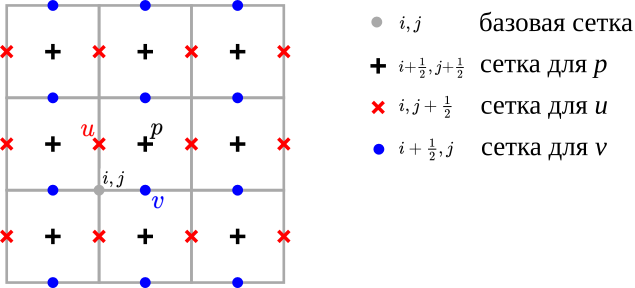
\includegraphics[width=0.6\linewidth]{staggered_grid.png}
\caption{Разнесённая сетка}
\label{fig:staggered_grid}
\end{figure}

Введём разбиение сетки:
$n_x$ -- количество ячеек в направлении $x$,
$n_y$ -- количество ячеек в направлении $y$.

Очевидно, что при использовании такого разнесённого шаблона,
количество точек, в которых заданы значения, будет
различным для разных параметров.
Так количество узловых значений давления будет равно $n_x \times n_y$,
продольной скорости $u$ -- $(n_x+1) \times n_y$, а поперечной $v$ -- $n_x \times (n_y+1)$.

Использование такого расположения узловых точек
даёт преимущество при аппроксимации
первых производных. Так, конечная разность
\begin{equation*}
\left.\dfr{p}{x}\right|_{i, j+\tfrac12} = \frac{p_{i+\tfrac12,j+\tfrac12} - p_{i-\tfrac12,j+\tfrac12}}{h_x} + o(h_x^2)
\end{equation*}
будем симметричной в узле $i,j+\tfrac12$, где задана
компонента скорости $u$, и поэтому будет иметь там второй порядок точности.

Выражения \eqref{eq:ns2d_ustar}, \eqref{eq:ns2d_uprime_approx} аппроксимируются
на сетке для $u$, выражения \eqref{eq:ns2d_vstar}, \eqref{eq:ns2d_vprime_approx} -- 
на сетке для $v$, а \eqref{eq:ns2d_pprime_diff} -- на сетке для $p$.

Введём сквозную линейную нумерацию узлов сетки: нулевой узел разположим в левом нижнем углу,
далее будем индексировать слева направа и потом снизу вверх.
Для основной сетки перевод двумерного индекса $i,j$ в сквозной индекс будет проводится по формуле
\begin{equation}
    \label{eq:ns2d_kij}
    k(i,j) = j(n_x+1)+i.
\end{equation}
Для сеток, на которых заданы сеточные параметры, такой перевод примет вид
\begin{align}
    \label{eq:ns2d_kipjp}
    &k(i+\tfrac12,j+\tfrac12) = jn_x + i, \quad - \; \text{сетка для давления } p\\[10pt]
    \label{eq:ns2d_kijp}
    &k(i,j+\tfrac12) = j(n_x+1) + i, \quad - \;  \text{сетка для продольной скорости } {\color{red} u} \\[10pt]
    \label{eq:ns2d_kipj}
    &k(i+\tfrac12,j) = jn_x + i, \quad - \; \text{сетка для поперечной скорости } {\color{blue} v}
\end{align}

\subsubsubsection{Уравнения движения}

Запишем конечноразностную аппроксимацию уравнения \eqref{eq:ns2d_ustar} для пробной скорости $u^*$ в ``красных'' узлах сетки
$\left(i, j+\tfrac12\right)$:

\begin{align}
    \label{eq:ns2d_ustar_discr}
    u^*_{i, j+\tfrac12} 
        &+ \frac{\tau}{h_x}
          \left(
            \left(u u^*\right)_{i+\tfrac12,j+\tfrac12}-
            \left(u u^*\right)_{i-\tfrac12,j+\tfrac12}
          \right)  \\[10pt]
    \nonumber
        &+ \frac{\tau}{h_y}
          \left(
            \left(v u^*\right)_{i,j+1}-
            \left(v u^*\right)_{i,j}
          \right)   \\[10pt]
    \nonumber
       &-\frac{1}{\Ren}\frac{\tau}{h_x^2}
          \left(
            u^*_{i-1,j+\tfrac12} - 2 u^*_{i,j+\tfrac12} + u^*_{i+1,j+\tfrac12}
          \right)   \\[10pt]
    \nonumber
       &-\frac{1}{\Ren}\frac{\tau}{h_y^2}
          \left(
            u^*_{i,j-\tfrac12} - 2 u^*_{i,j+\tfrac12} + u^*_{i,j+\tfrac32}
          \right)   \\[10pt]
    \nonumber
       &= u_{i,j+\tfrac12} -\frac{\tau}{h_x}\left(p_{i+\tfrac12,j+\tfrac12} - p_{i-\tfrac12,j+\tfrac12}\right).
\end{align}

В приведённом выражении
за исключением конвективных слагаемых вида $u u$ все остальные
сеточные вектора используются на своих сетках.
Конвективные слагаемые распишем через полусуммы вида:
\begin{equation*}
    u_{i+\tfrac12} = \frac{u_{i} + u_{i+1}}{2} + o(h^2)
\end{equation*}

Тогда
\begin{align*}
    \left(u u^*\right)_{i+\tfrac12,j+\tfrac12} =&
        \left(u_{i+\tfrac12,j+\tfrac12} \vphantom{u^*_{\tfrac12}}\right)\left(u^*_{i+\tfrac12,j+\tfrac12}\right) =
        \frac14 \left(u_{i, j+\tfrac12} + u_{i+1,j+\tfrac12}\vphantom{u^*_{\tfrac12}}\right)
                \left(u^*_{i, j+\tfrac12} + u^*_{i+1,j+\tfrac12}\right), \\[10pt]
    \left(u u^*\right)_{i-\tfrac12,j+\tfrac12} =&
        \frac14 \left(u_{i, j+\tfrac12} + u_{i-1,j+\tfrac12}\vphantom{u^*_{\tfrac12}}\right)
                \left(u^*_{i, j+\tfrac12} + u^*_{i-1,j+\tfrac12}\right), \\[10pt]
    \left(v u^*\right)_{i,j+1} =&
        \frac14 \left(v_{i+\tfrac12, j+1} + v_{i-\tfrac12,j+1}\vphantom{u^*_{\tfrac12}}\right)
                \left(u^*_{i, j+\tfrac32} + u^*_{i,j+\tfrac12}\right), \\[10pt]
    \left(v u^*\right)_{i,j} =&
        \frac14 \left(v_{i+\tfrac12, j} + v_{i-\tfrac12,j}\vphantom{u^*_{\tfrac12}}\right)
                \left(u^*_{i, j+\tfrac12} + u^*_{i,j-\tfrac12}\right).
\end{align*}

Схему \eqref{eq:ns2d_ustar_discr} можно записать в виде системы линейных уравнений вида
\begin{equation}
    \label{eq:ns2d_ustar_slae}
    A^u u^* = b^{u}.
\end{equation}
Сеточная матрица $A^u$ будет иметь $(n_x+1)n_y$ строк.
Для строки, соответствующей $\left(i,j+\tfrac12\right)$ узлу ненулевыми будут столбцы,
соответствующие узлам:
\begin{itemize}
\item $\left(i,j+\tfrac12\right)$,
\item $\left(i+1,j+\tfrac12\right)$,
\item $\left(i-1,j+\tfrac12\right)$,
\item $\left(i,j+\tfrac32\right)$,
\item $\left(i,j-\tfrac12\right)$.
\end{itemize}

В случае использования стандартной нумерации узлов структурированной сетки,
когда нулевой индекс соответствуют левому нижнему узлу и далее нумерация идёт
с быстрым индексом $i$, то матрица будет пятидиагональной.


Подставим полученные выражения в конвективную часть выражения \eqref{eq:ns2d_ustar_discr}.
Множитель при диагональном элементе $u^*_{i,j+\tfrac12}$ будет равен:
\begin{align*}
        \frac{\tau}{4}\Biggl(
         \underbrace{\frac{u_{i,j+\tfrac12} - u_{i-1,j+\tfrac12}}{h_x}}_{\left.\ddfr{u}{x}\right|_{i-\tfrac12,j+\tfrac12}}
        +\underbrace{\frac{u_{i+1,j+\tfrac12} - u_{i,j+\tfrac12}}{h_x}}_{\left.\ddfr{u}{x}\right|_{i+\tfrac12,j+\tfrac12}}
        +\underbrace{\frac{v_{i+\tfrac12,j+1} - v_{i+\tfrac12,j}}{h_y}}_{\left.\ddfr{v}{y}\right|_{i+\tfrac12,j+\tfrac12}}
        +\underbrace{\frac{v_{i-\tfrac12,j+1} - v_{i-\tfrac12,j}}{h_y}}_{\left.\ddfr{v}{y}\right|_{i-\tfrac12,j+\tfrac12}}
        \Biggr)
\end{align*}

Сумма первого и четвёртого слагаемых представляет собой разностный
аналог уравнения неразрывности \eqref{eq:ns2d_semi_div}, записанной для ``чёрного'' узла
сетки $i-\tfrac12, j+\tfrac12$ относительно компонент
скорости с предыдущей итерации.
Как было сказано ранее,
в настоящем алгоритме
уравнение неразрывности для итоговых по результатам итерации скорости в этих узлах выполняется точно.
Поэтому эта сумма в точности будет равна нулю. Аналогичный результат получится
и для суммы второго и третьего слагаемых. Отсюда следует вывод, что
конвективное слагаемое не даёт вклад в диагональ итоговой матрицы (как и следовало ожидать от симметричной аппроксимации).

Окончательно запишем все пять ненулевых вхождений в строку матрицы:
\begin{align}
    \label{eq:ns2d_au}
    A^u\left[
        k\left(i,j+\tfrac12\right),
        k\left(i,j+\tfrac12\right)\right]
        &= 1 + \frac{2\tau}{\Ren}\left(\frac{1}{h_x^2} + \frac{1}{h_y^2}\right)
        \quad - \;\text{основная диагональ}, \\[10pt]
    \nonumber
    A^u\left[
        k\left(i,j+\tfrac12\right),
        k\left(i+1,j+\tfrac12\right)\right]
        &= -\frac{\tau}{\Ren}\frac{1}{h_x^2}
           +\frac{\tau}{4h_x}\left(u_{i,j+\tfrac12}+u_{i+1,j+\tfrac12}\right)
        \quad - \;\text{первая верхняя диагональ}, \\[10pt]
    \nonumber
    A^u\left[
        k\left(i,j+\tfrac12\right),
        k\left(i-1,j+\tfrac12\right)\right]
        &= -\frac{\tau}{\Ren}\frac{1}{h_x^2}
           -\frac{\tau}{4h_x}\left(u_{i,j+\tfrac12}+u_{i-1,j+\tfrac12}\right)
        \quad - \;\text{первая нижняя диагональ}, \\[10pt]
    \nonumber
    A^u\left[
        k\left(i,j+\tfrac12\right),
        k\left(i,j+\tfrac32\right)\right]
        &= -\frac{\tau}{\Ren}\frac{1}{h_y^2}
           +\frac{\tau}{4h_y}\left(v_{i+\tfrac12,j+1}+v_{i-\tfrac12,j+1}\right)
        \quad - \;\text{вторая верхняя диагональ}, \\[10pt]
    \nonumber
    A^u\left[
        k\left(i,j+\tfrac12\right),
        k\left(i,j-\tfrac12\right)\right]
        &= -\frac{\tau}{\Ren}\frac{1}{h_y^2}
           -\frac{\tau}{4h_y}\left(v_{i+\tfrac12,j}+v_{i-\tfrac12,j}\right)
        \quad - \;\text{вторая нижняя диагональ}.
\end{align}
Здесь $k(i,j)$ -- функция перевода двумерного индекса в сквозной \eqref{eq:ns2d_kijp}.

Аналогичные выкладки для второго из уравнений движения \eqref{eq:ns2d_vstar}
дают систему уравнений
\begin{equation}
    \label{eq:ns2d_vstar_slae}
    A^v v^* = b^{v},
\end{equation}
элементы пятидиагональной матрицы которой имеют вид
\begin{align}
    \label{eq:ns2d_av}
    A^v\left[
        k\left(i+\tfrac12,j\right),
        k\left(i+\tfrac12,j\right)\right]
        &= 1 + \frac{2\tau}{\Ren}\left(\frac{1}{h_x^2} + \frac{1}{h_y^2}\right)
        \quad - \;\text{основная диагональ}, \\[10pt]
    \nonumber
    A^v\left[
        k\left(i+\tfrac12,j\right),
        k\left(i+\tfrac32,j\right)\right]
        &= -\frac{\tau}{\Ren}\frac{1}{h_x^2}
           +\frac{\tau}{4h_x}\left(u_{i+1,j+\tfrac12}+u_{i+1,j-\tfrac12}\right)
        \quad - \;\text{первая верхняя диагональ}, \\[10pt]
    \nonumber
    A^v\left[
        k\left(i+\tfrac12,j\right),
        k\left(i-\tfrac12,j\right)\right]
        &= -\frac{\tau}{\Ren}\frac{1}{h_x^2}
           -\frac{\tau}{4h_x}\left(u_{i,j+\tfrac12}+u_{i,j-\tfrac12}\right)
        \quad - \;\text{первая нижняя диагональ}, \\[10pt]
    \nonumber
    A^v\left[
        k\left(i+\tfrac12,j\right),
        k\left(i+\tfrac12,j+1\right)\right]
        &= -\frac{\tau}{\Ren}\frac{1}{h_y^2}
           +\frac{\tau}{4h_y}\left(v_{i+\tfrac12,j}+v_{i+\tfrac12,j+1}\right)
        \quad - \;\text{вторая верхняя диагональ}, \\[10pt]
    \nonumber
    A^v\left[
        k\left(i+\tfrac12,j\right),
        k\left(i+\tfrac12,j-1\right)\right]
        &= -\frac{\tau}{\Ren}\frac{1}{h_y^2}
           -\frac{\tau}{4h_y}\left(v_{i+\tfrac12,j}+v_{i+\tfrac12,j-1}\right)
        \quad - \;\text{вторая нижняя диагональ}.
\end{align}
Правая часть аппроксимируется в виде
\begin{equation*}
    b^{v^*}[k(i+\tfrac12, j)] = 1 - \frac{\tau}{h_y}\left(p_{i+\tfrac12, j+1} - p_{i+\tfrac12,j}\right).
\end{equation*}
Используется функция перевода двумерного индекса в сквозной из \eqref{eq:ns2d_kipj}.

\subsubsubsection{Уравнение для поправки давления}
Распишем уравнение \eqref{eq:ns2d_pprime_diff}
на ``чёрной'' сетке методом конечных разностей.
Для первого слагаемого получим
\begin{equation}
\label{eq:ns2d_d2pdx2}
\begin{array}{ll}
\left.\ddfr{}{x}\left(d^u \ddfr{p'}{x}\right) \right|_{i+\tfrac12, j+\tfrac12}
    &\approx
        \dfrac{1}{h_x}\left(
            d^u_{i+1, j+\tfrac12} \left. \ddfr{p'}{x} \right|_{i+1, j+\tfrac12} -
            d^u_{i, j+\tfrac12} \left. \ddfr{p'}{x} \right|_{i, j+\tfrac12}
        \right) \\[10pt]

    &=
        \dfrac{1}{h_x}\left(
            d^u_{i+1, j+\tfrac12} \dfrac{p'_{i+\tfrac32,j+\tfrac12} - p'_{i+\tfrac12,j+\tfrac12}}{h_x} - 
            d^u_{i, j+\tfrac12}  \dfrac{p'_{i+\tfrac12,j+\tfrac12} - p'_{i-\tfrac12,j+\tfrac12}}{h_x}
        \right).
\end{array}
\end{equation}
Аналогично расписываются остальные слагаемые. В результате получим систему линейных уравнений вида
\begin{equation}
    \label{eq:ns2d_pprime_slae}
    A^p p' = b^p,
\end{equation}
где ненулевые коэффициенты пятидиагональной матрицы примут вид
\begin{align}
    \label{eq:ns2d_ap}
    A^p[k(i+\tfrac12, j+\tfrac12), k(i+\tfrac12, j+\tfrac12)] =&
        \frac{1}{h_x^2}\left( d^u_{i+1,j+\tfrac12} + d^u_{i,j+\tfrac12} \right)
        +\frac{1}{h_y^2}\left( d^v_{i+\tfrac12,j} + d^v_{i+\tfrac12,j+1} \right), \\[10pt]
    \nonumber
    A^p[k(i+\tfrac12, j+\tfrac12), k(i+\tfrac32, j+\tfrac12)] =&
        -\frac{1}{h_x^2}d^u_{i+1,j+\tfrac12}, \\[10pt]
    \nonumber
    A^p[k(i+\tfrac12, j+\tfrac12), k(i-\tfrac12, j+\tfrac12)] =&
        -\frac{1}{h_x^2}d^u_{i,j+\tfrac12}, \\[10pt]
    \nonumber
    A^p[k(i+\tfrac12, j+\tfrac12), k(i+\tfrac12, j+\tfrac32)] =&
        -\frac{1}{h_y^2}d^v_{i+\tfrac12,j+1}, \\[10pt]
    \nonumber
    A^p[k(i+\tfrac12, j+\tfrac12), k(i+\tfrac12, j-\tfrac12)] =&
        -\frac{1}{h_y^2}d^v_{i+\tfrac12,j}.\\[10pt]
\end{align}
Столбец свободных членов аппроксимируется в виде
\begin{equation}
    \label{eq:ns2d_bp}
    b^p[k(i+\tfrac12,j+\tfrac12)] = 
        -\frac{1}{\tau}
        \left(
              \frac{u^*_{i+1,j+\tfrac12} - u^*_{i,j+\tfrac12}}{h_x}
            + \frac{v^*_{i+\tfrac12,j+1} - v^*_{i+\tfrac12,j}}{h_y}
        \right).
\end{equation}
Здесь используется функция перевода двумерного индекса в сквозной из $\eqref{eq:ns2d_kipjp}$.

Далее определим значения $d^u, d^v$.
Согласно идее алгоритма SIMPLE $d^u$ должна
быть такой функцией, которая максимально приближает
выражение \eqref{eq:ns2d_uprime} к \eqref{eq:ns2d_uprime_approx}.

Пространственная аппроксимация выражения \eqref{eq:ns2d_uprime}
приводит к системе уравнений
\begin{equation*}
    A^u u' = -\tau\dfr{p'}{x}
\end{equation*}
где матрица $A^u$ -- та же самая матрица, которая использовалась
при аппроксимации уравнения движения \eqref{eq:ns2d_ustar_discr}.

Сравнивая предыдущее выражение с \eqref{eq:ns2d_uprime_approx}
сделаем вывод, что $d^u$ должна быть такой, чтобы
\begin{equation*}
    d^u \dfr{p'}{x} \approx \left(A^u\right)^{-1} \dfr{p'}{x}.
\end{equation*}
То есть поэлементное умножение сеточного вектора ${d^u}$ 
на другой вектор
должно действовать похоже на умножение обратной к $A^u$ матрицы на этот же самый вектор.

Исходя из свойств матрицы $A^u$ \eqref{eq:ns2d_au} можно
положить 
\begin{equation}
    \label{eq:ns2d_du}
    d^u = \left({\rm diag}\left(A^u\right)\right)^{-1} = 
        \left(1 + \frac{2\tau}{\Ren}\left(\frac{1}{h_x^2} + \frac{1}{h_y^2}\right)\right)^{-1}
\end{equation}
и аналогично из \eqref{eq:ns2d_av}
\begin{equation}
    \label{eq:ns2d_dv}
    d^v = \left({\rm diag}\left(A^v\right) \right)^{-1}= 
        \left(1 + \frac{2\tau}{\Ren}\left(\frac{1}{h_x^2} + \frac{1}{h_y^2}\right)\right)^{-1}.
\end{equation}
Равентство коэффициентов $d^u = d^v$ -- следствие использования симметричной
аппроксимации конвективного слагаемого в уравнениях движения.

Таким образом мы получили выражения для коэффициентов уравнения для поправки давления,
которые зависят только от разбиения сетки.
В случае, если разбиение равномерное ($h_x = {\rm const}, h_y = {\rm const}$),
то все значения коэффициентов одинаковы.
Однако, для неравномерных разбиений, они будут зависеть
от пространства и задаваться на ``красной'' (для $d^u$) и ``синей'' (для $d^v$)
сетках.

В результате использования \eqref{eq:ns2d_du}, \eqref{eq:ns2d_dv} левая часть системы уравнений \eqref{eq:ns2d_pprime_slae}
будет постоянна на всех итерациях, что удобно для инициализации алгебраических решателей этой системы
(можно провести инициализацию один раз до начала счёта).

Это отличает эту систему от двух других систем, возникающих
из аппроксимации уравнений движения \eqref{eq:ns2d_ustar_slae}, \eqref{eq:ns2d_vstar_slae},
левые части которых зависят от значений с предыдущих
итерационных слоёв. Этот момент обуславливает выбор
решателей для этих систем, которые в эффективных гидродинамических кодах обычно
отличаются, от решателя для системы \eqref{eq:ns2d_pprime_slae}.


\subsubsubsection{Уравнение для поправки скорости}
И наконец рассмотрим аппроксимацию выражений \eqref{eq:ns2d_uprime_approx},
\eqref{eq:ns2d_vprime_approx}, которые примут явный вид
\begin{align}
    \label{eq:ns2d_uprime_discr}
    u'_{i,j+\tfrac12} = -\tau d^u_{i,j+\tfrac12} \frac{p'_{i+\tfrac12,j+\tfrac12} - p'_{i-\tfrac12, j+\tfrac12}}{h_x}, \\[10pt]
    \label{eq:ns2d_vprime_discr}
    v'_{i+\tfrac12,j} = -\tau d^v_{i+\tfrac12,j} \frac{p'_{i+\tfrac12,j+\tfrac12} - p'_{i+\tfrac12, j-\tfrac12}}{h_x}.
\end{align}

\subsubsubsection{Учёт граничных условий}
\label{sec:simple-bc}

Для уравнений Навье-Стокса на каждой границе расчётной области
требуется столько условий, сколько есть уравнений движения.
Для двумерной задачи \cref{eq:ns2d_u,eq:ns2d_div,eq:ns2d_v}
нужно задать два граничных условия.

При использовании разнесённой сетки граница области проходит
по граням основной сетки. 
На нижней и верхней границах расчётной области
присутствуют узлы для $v$, но отсутствуют
узлы для $u$.
На правой и левой границах, наоборот,
есть узлы с заданными компонентами $u$,
но нет узлов с компонентами $v$.
Узловые значения для давления $p$
никогда не бывают граничными.

Для простоты пока будем рассматривать только случай с заданными значениями
двух компонент скорости на каждой из границ задачи:
\begin{align*}
    &\left. u(x, y) \right|_{x,y\in\Gamma} = u^\Gamma(x, y), \\
    &\left. v(x, y) \right|_{x,y\in\Gamma} = v^\Gamma(x, y).
\end{align*}

В схеме SIMPLE частные граничные условия 
для скорости учитываются при решении задачи
для пробных скоростей $u^*, v^*$.
Тогда для поправки скорости $u', v'$ на границах
будут справедливы соответствующие однородные граничные условия (нулевые значения в нашем случае):

\begin{align}
    \label{eq:ns2d_usplit_bc}
    &\left. u^*(x, y) \right|_{x,y\in\Gamma} = u^\Gamma(x, y), \\
    \nonumber
    &\left. v^*(x, y) \right|_{x,y\in\Gamma} = v^\Gamma(x, y), \\
    \nonumber
    &\left. u'(x, y) \right|_{x,y\in\Gamma} = 0,\\
    \nonumber
    &\left. v'(x, y) \right|_{x,y\in\Gamma} = 0.
\end{align}

Для учёта граничных условий по скорости требуется модифицировать
системы линейных уравнений \eqref{eq:ns2d_ustar_slae}, \eqref{eq:ns2d_vstar_slae}.

Рассмотрим нижнюю границу $j=0$.

На нижней границе явно присутствуют узлы ``синей'' сетки.
Значит можно явно установить значения для скорости $v$
путём постановки нулей с единицой на диагонали в строке матрицы и отнесением необходимого
граничного значение в правый вектор столбец системы \eqref{eq:ns2d_vstar_slae}:
\begin{align}
    \label{eq:ns2d_bc1}
    &A^v[k(i+\tfrac12, 0), s] = \delta_{ks}, \quad \forall i, \; \forall s\\[10pt]
    \nonumber
    &b^{v}[k(i+\tfrac12, 0)] = v^\Gamma.
\end{align}
Такая модификация просто заменяет $k(i+\tfrac12, 0)$ -ое уравнение
системы \eqref{eq:ns2d_vstar_slae} на выражение
\begin{equation*}
    v^*_{i+\tfrac12, 0} = v^\Gamma.
\end{equation*}

Узлов для компонет $u$ на нижней границе нет.
Рассмотрим первый ряд точек ``красной'' сетки: $(i, \tfrac12)$.
Если бы мы захотели заполнить коэффициенты системы
линейных уравнений \eqref{eq:ns2d_ustar_slae}
по выведенным выше формулам \eqref{eq:ns2d_au}
для узла, расположенного в этом ряду, мы бы столкнулись
с необходимостью установки значения в фиктивную колонку:
последнее из уравнений \eqref{eq:ns2d_au}
предписывает нам установить значение по адресу
$[k(i, \tfrac12), k(i, -\tfrac12)]$, который, очевидно, не присутствует в матрице.

Действительно, $k(i,\tfrac12)$-ая строка системы уравнений \eqref{eq:ns2d_au}
имеет вид
\begin{equation}
    \label{eq:ns2d_au_low}
      D    u^*_{i, \tfrac12}
    + U^1  u^*_{i+1, \tfrac12}
    + L^1  u^*_{i-1, \tfrac12}
    + U^2 u^*_{i, \tfrac32}
    + L^2 u^*_{i, -\tfrac12} 
    = b^u_{i, \tfrac12},
\end{equation}
где $D$ -- коэффициент с основной диагонали, $U^{1,2}, L^{1,2}$ -- 
коэффициенты с двух верхних и двух нижних диагоналей, вычисляемые по формулам \eqref{eq:ns2d_au}.
Вторая нижняя диагональ у этой строки матрицы отсутствует.
Она соответствует вкладу от узла $(i, -\tfrac12)$, который лежит вне области расчёта, на полшага ниже
нижней границе.

Тем не менее, такой фиктивный узел мы можем 
использовать для записи аппроксимации
\begin{equation*}
    u^*_{i,0} = u^\Gamma = \frac{u^*_{i,\tfrac12} + u^*_{i, -\tfrac12}}{2} + o(h_x^2).
\end{equation*}
или
\begin{equation*}
    u^*_{i, -\tfrac12} \approx 2u^\Gamma - u^*_{i,\tfrac12}.
\end{equation*}

Подставляя это выражение в строку \eqref{eq:ns2d_au_low} получим
\begin{equation*}
      (D - L^2) u^*_{i, \tfrac12}
    + U^1       u^*_{i+1, \tfrac12}
    + L^1       u^*_{i-1, \tfrac12}
    + U^2       u^*_{i, \tfrac32}
    = b^u_{i, \tfrac12} + 2 u^\Gamma.
\end{equation*}

Таким образом, добавление коэффициента в фиктивную колонку строки матрицы при
наличие условия первого рода на границе равносильно
вычитанию этого коэффициента из диагонального элемента этой строки
и вычитанием удвоенного граничного значения из правой части.
В случае нижней границы получим
\begin{align}
    \label{eq:ns2d_bc2}
    &A^u[k(i, \tfrac12), k(i, \tfrac12)] \mathrel{-}= A^u[k(i, -\tfrac12)], \\[10pt]
    \nonumber
    &b^u[k(i, \tfrac12)] \mathrel{-}= 2 u^\Gamma.
\end{align}

Приёмы \eqref{eq:ns2d_bc1}, \eqref{eq:ns2d_bc2}
используются и на остальных границах для
постановки граничных условий для скорости.

При сборке системы линейных уравнений для
поправки давления \eqref{eq:ns2d_pprime_slae}
так же возникает проблема с обращением
к фиктивным узлам. Например, при рассмотрении левой стенки ($i=0$
третье из уравнений \eqref{eq:ns2d_ap} описывает
несуществующий столбец $k(-\tfrac12, j+\tfrac12)$.
Если обратиться к выражению \eqref{eq:ns2d_d2pdx2},
то будет видно, что это слагаемое пришло в результате
расписывания граничной производной $p'$,
которая, исходя из выражения \eqref{eq:ns2d_uprime_approx} пропорциональна граничному значению $u'$,
то есть, вспоминая \eqref{eq:ns2d_usplit_bc}, равна нулю:
\begin{equation*}
\left. \dfr{p'}{x} \right|_{0,j+\tfrac12} = -\frac{1}{\tau d^u} u'_{0,j+\tfrac12} = 0.
\end{equation*}

То есть добавлять слагаемые, соответствующие фиктивным узлам, в матрицу $A^p$ не нужно.
Не нарушая общности выведённых ранее выражений \eqref{eq:ns2d_ap},
просто модифицируем значения коэффициентов $d^u, d^v$:
\begin{align}
    \label{eq:ns2d_bc3}
    d^u_{0, j+\tfrac12} = d^u_{n_x+1, j+\tfrac12} = 0, \\[10pt]
    \nonumber
    d^v_{i+\tfrac12, 0} = d^u_{i+\tfrac12, n_y+1} = 0.
\end{align}

В исходных уравнениях
\eqref{eq:ns2d_u}-\eqref{eq:ns2d_div}
давление присутствует только в виде своих производных.
Если в задаче нигде не задано явное граничное условие
для давления, то решение для давления
будет определено только с точностью до константы.
Чтобы убрать эту неопределённость
рекомендуется явно положить давление нулю
в любом узле. Например, в случае нулевого узла,
по аналогии с \eqref{eq:ns2d_bc1} запишем:
\begin{align}
    \label{eq:ns2d_bc4}
    &A^p[k(\tfrac12, \tfrac12), s] = \delta_{ks}, \\[10pt]
    \nonumber
    &b^{p}[k(\tfrac12, \tfrac12)] = 0.
\end{align}

\subsubsection{Оптимальные значения параметров алгоритма SIMPLE}

Введем обозначение
\begin{equation*}
\label{eq:ns2d-simple-e}
E = \frac{4\tau}{\Ren\,\bar h^2}
\end{equation*}
где ${\bar h^2}$ -- среднее гармоническое значение шага, определяемое как
$$
\bar h^2 = \frac{2\,h_x^2\,h_y^2}{h_x^2 + h_y^2}.
$$
Значение $E$ -- есть диагональное компонента матрицы диффузии
в аппроксимированных уравнениях движения (второе слагаемое в правой части первой формулы \cref{eq:ns2d_au}).

При независимом задании релаксаций по скорости и давлению,
оптимальной сходимости соответствуют значения
\begin{align*}
&E = 1 \hence \tau = \frac{\Ren \,\bar h^2}{4}, \\
&\alpha_p = 0.8.
\end{align*}
Ещё более эффективной сходимости соответствуют параметры
\begin{equation}
\label{eq:ns2d-simplec}
E \approx 4, \quad \alpha_p = \frac{1}{1+E}.
\end{equation}
Это выражение соответствует алгоритму SIMPLEC (согласованный алгоритм, SIMPLE Consistent).

\subsection{Программа для расчёта течения в каверне по схеме SIMPLE}
\label{sec:prog-cavity2}

\subsubsection{Постановка задачи}

Для иллюстрации работы алгоритма рассмотрим задачу о 
течении в каверне. Постановку задачи представлена на \figref{fig:cavity}.

\begin{figure}[h]
\centering
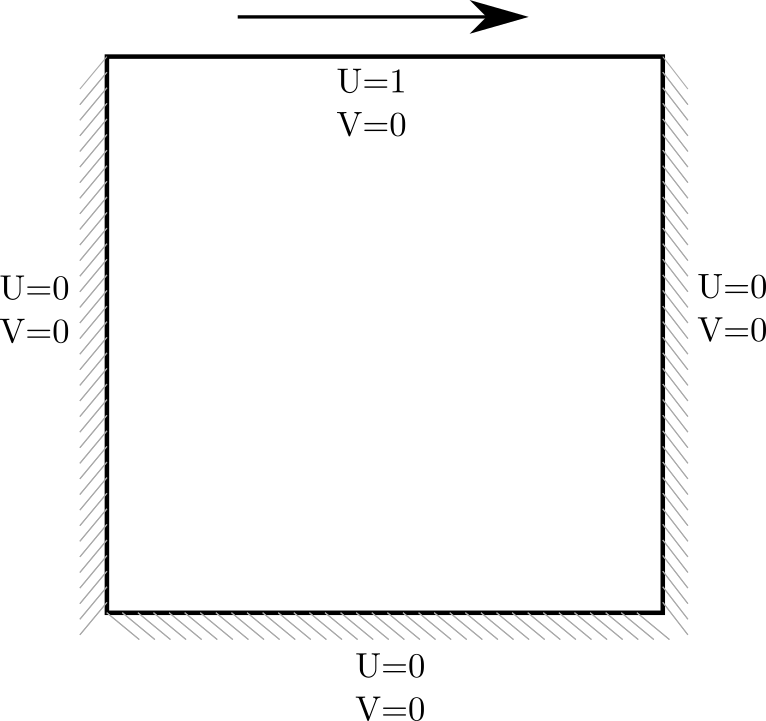
\includegraphics[width=0.4\linewidth]{cavity2d.png}
\caption{Область расчёта задачи о каверне}
\label{fig:cavity}
\end{figure}

Задача реализована в тесте \ename{[cavity2-simple]} в файле \ename{cavity_simple_test.cpp}.

Программа проводит итерации стартуя от начального нулевого состояния
$u=v=p=0$ до тех пор, пока невязка не достигнет заданного порога.
На каждой итерации поле давления и векторное поле скорости сохраняются
на основной сетке в файл \ename{cavity2.vtk.series}.

Итоговый результат (для $\eps=10^{-2}$) представлен на \figref{fig:cavity-result}.

\begin{figure}[h]
\centering
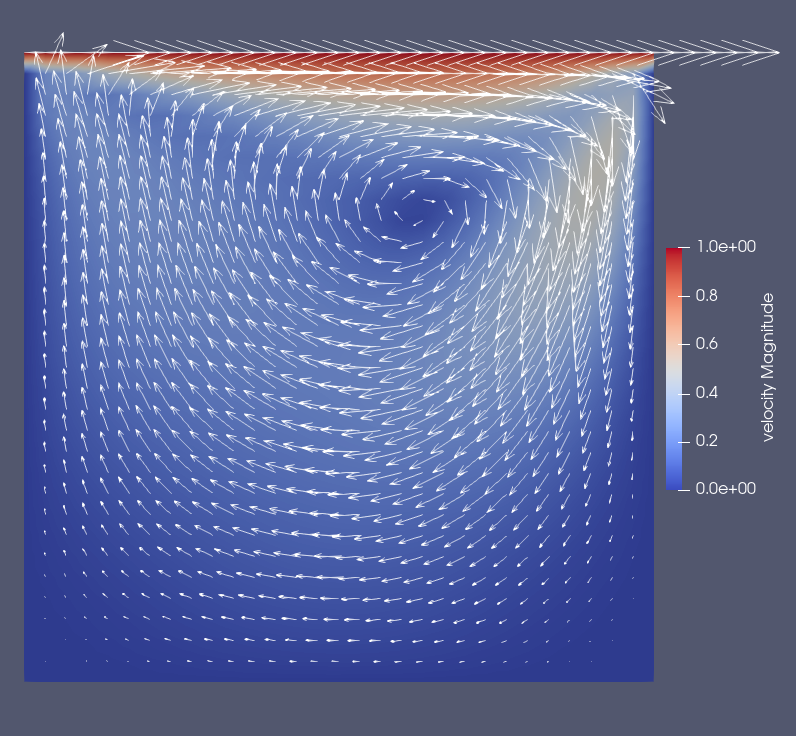
\includegraphics[width=0.7\linewidth]{cavity2d-result.png}
\caption{Область расчёта задачи о каверне}
\label{fig:cavity-result}
\end{figure}

Для отображения вектора поля скорости в Paraview см. справку в \ref{sec:paraview-glyph}.

Для работы с разнесённой сеткой в классе \cvar{cfd::RegularGrid2D}
представлены функции
\begin{itemize}
\item \cvar{cfd::RegularGrid2D::cell_centered_grid()}  -- построить сетку по центрам ячеек (``чёрную'' сетку для $p$),
\item \cvar{cfd::RegularGrid2D::xface_centered_grid()} -- построить сетку по центрам $x$-граней (``синюю'' сетку для $v$),
\item \cvar{cfd::RegularGrid2D::yface_centered_grid()} -- построить сетку по центрам $y$-граней (``красную'' сетку для $u$),
\end{itemize}

и функции перевода индексов
\begin{itemize}
\item \cvar{cfd::RegularGrid2D::cell_centered_grid_index_ip_jp} -- посчитать линейный индекс ``чёрной'' сетки \eqref{eq:ns2d_kipjp},
\item \cvar{cfd::RegularGrid2D::xface_grid_index_ip_j} -- посчитать линейный индекс ``синей'' сетки \eqref{eq:ns2d_kipj},
\item \cvar{cfd::RegularGrid2D::yface_grid_index_i_jp} -- посчитать линейный индекс ``красной'' сетки \eqref{eq:ns2d_kijp}.
\end{itemize}

\subsubsection{Функция верхнего уровня}
\clisting{open}{"test/cavity_simple_test.cpp"}
\clisting{line}{"[cavity2-simple]"}

Сначала устанавливаются параметры задачи:
число Рейнолдса,
\clisting{line}{"Re"}
параметры алгоритма SIMPLE,
\clisting{lines-range}{"tau", "alpha"}
разбиение сетки, 
\clisting{line}{"n_cells"}
максимальное количество итераций 
\clisting{line}{"max_it"}
и значение невязки, при котором итерации прекращаются
\clisting{line}{"double eps"}

Затем происходит инициализация решателя, который
определён в классе \cvar{Cavity2DSimpleWorker}
\clisting{line}{"Cavity2DSimpleWorker"}
и параметров сохранения. Здесь
первым параметром является флаг сохранения
точных сеточных значений, который установлен в \cvar{false},
а также имя файла с итоговым результатом.
Таким образом сохраняться будет только решение,
интерполированное на основную сетку.
Для целей отладки программы (для просмотра действительных, не интерполированных полей решения)
следует первый флаг установить в \cvar{true}. Тогда помимо \ename{cavity2.vtk.series}, будут
создаваться также файлы \ename{cavity2-u}, \ename{cavity2-v}, \ename{cavity2-p}.
\clisting{until}{"_saver"}

Потом происходит установка начальных значений искомых сеточных векторов: $u=v=p=0$
\clisting{lines-range}{"u_init", "set_uvp"}

и начинается итерационный процесс.
\clisting{line}{"for"}

Внутри цикла
выполняется шаг итерационного процесса, который
возвращает значение итоговой невязки в переменную \cvar{nrm}.
\clisting{line}{"step"}

На печать выводится индекс итерации, значение невязки и значение давления в правом верхнем узле (для контроля сходимости)
\clisting{line}{"cout"}

Сохраняется состояние решателся на пройденную итерацию
\clisting{line}{"save_current"}

и производится проверка на сходимость
\clisting{block}{"if (nrm < eps)"}

В конце производится проверка: при установленных параметрых решение
должно сойтись за 9 итераций:
\clisting{line}{"CHECK"}

\subsubsection{Поля класса решателя}
\clisting{to-start}{}
Класс \cvar{Cavity2DSimpleWorker} хранит в себе набор полей,
характеризующих состояние итерационного процесса.
Некоторые из этих полей (параметры решателя) постоянны (\cvar{const}) и
определяются непосредственно перед вызовом конструктора в инициализаторе. Другие
меняются с продвижением по итерациям.

Среди постоянных полей заданы 4 сетки: основная \cvar{_grid},
``чёрная'' сетка \cvar{_cc_grid} (cell-centered) для давления,
``красная'' сетка \cvar{_yf_grid} (y-face) для $u$,
``синяя'' сетка \cvar{_xf_grid} (x-face) для $v$ (\figref{fig:staggered_grid}).
\clisting{pass}{"private"}
\clisting{until}{"_yf_grid"}
Далее заданы скалярные параметры: число Рейнольдса, шаги сетки и параметры алгоритма SIMPLE
\clisting{until}{"_alpha_p"}

Далее следуют сеточные вектора, характеризующие текущее состояние решателя:
найденные на последней итерации давление и скорости.
\clisting{until}{"_v;"}

Также определяется данные для решения системы уравнений для нахождения $p'$ \eqref{eq:ns2d_pprime_slae}:
значения $d^u, d^u$, а так же инициализированный решатель системы уравнений.
Поскольку используется постоянные шаги по времени, $d^u, d^v$ являются скалярами.
\clisting{until}{"_p_prime_solver"}

Хранятся левая и правая части систем уравнений \eqref{eq:ns2d_ustar_slae}, \eqref{eq:ns2d_vstar_slae}
для определения пробных значений скорости и расчета невязки.
\clisting{until}{"_rhs_v;"}

Указатели на классы, помогающие сохранять найденные вектора в vtk - формат.
Эти классы инициализируются только в случае, если пользователь указал на 
необходимость сохранения.
\clisting{until}{"_writer_all;"}

\subsubsection{Инициализация решателя}
\clisting{to-start}{}

В секции инициализации конструктора
созаются сетки в единичном квадрате и переписываются параметры решения.
Далее в теле конструктора вычисляются значения
$d^u, d^v$ по формулам \eqref{eq:ns2d_du}, \eqref{eq:ns2d_dv}
и собирается решатель для $p'$. Как было указано ранее,
матрица системы $A^p$ не меняется
с продвижением по итерациям, поэтому этот решатель можно собрать один раз
до начала счёта.

\clisting{block}{"Cavity2DSimpleWorker::Cavity2DSimpleWorker"}

Начальные значения устанавливаются через вызов функции \cvar{set_uvp}.
Эти начальные значения будут использоваться в качестве значений
с предыдущего итерационного слоя на первой итерации.

В функции происходит переписывание переданных векторов
в приватные поля класса.
\clisting{lines-range}{"set_uvp", "_p"}

После этого данных в классе-решателе достаточно,
для сборки матриц $A^u, A^v$ и правых частей
$b^u, b^v$ для системы уравнений \eqref{eq:ns2d_ustar_slae}, \eqref{eq:ns2d_vstar_slae}.
\clisting{until}{"v_slae()"}

Если посмотреть на выражение для невязки \eqref{eq:ns2d_residual} убрав в нём крышки над переменными, то можно
убедится, что оно аппроксимируется в виде
\begin{equation*}
    r_u = \frac{1}{\tau}\left(A^u u - b^u\right).
\end{equation*}
Поэтому после сборки систем уравнений движения, можно вычислить невязку, характеризующую
отклонение установленного в этой процедуре решения от желаемого:
\clisting{until-close}{}

\subsubsection{Шаг итерации SIMPLE}
\clisting{to-start}{}
Осуществляется в процедуре
\clisting{block}{"double Cavity2DSimpleWorker::step()"}
и представляет собой буквальное пошаговое следование алгоритму SIMPLE (\ref{sec:simple-algo}).
В конце опять вызывается функция \cvar{set_uvp} для сборки матриц для следующей итерации
и подсчёта невязки на текущей итерации.

\subsubsection{Сборка системы уравнений для поправки давления}
\clisting{to-start}{}

Сборка системы уравнений \eqref{eq:ns2d_pprime_slae}
осуществляется в процедуре
\clisting{line}{"void Cavity2DSimpleWorker::assemble_p_prime_solver()"}
Сборка происходит с использованием матрицы формата \cvar{cfd::LodMatrix},
удобного для непоследовательной записи.
\clisting{until}{"LodMatrix"}
Заполнение происходит в цикле по раздвоенным индексам $ij$
``чёрной'' сетки для давления:
\clisting{until}{"size_t i"}
Внутри цикла устанавливаются флаги, характеризующие граничный статус текущего узла
\clisting{until}{"is_top"}
Вычисляется значение сквозного индекса по формуле \eqref{eq:ns2d_kipjp}
\clisting{until}{"ind0"}
и значения коэффициентов в формулах \eqref{eq:ns2d_ap}. Поскольку
сетка равномерная, эти значения не меняются для разных узлов
\clisting{until}{"coef_y"}
Далее формулы \eqref{eq:ns2d_ap}
применяются для заполнения матриц
с учётом аппроксимированного граничного условия \eqref{eq:ns2d_bc3}.
Так, запись
\clisting{until-close}{}
для всех неправых узлов с линейным индексом \cvar{ind0} вычисляет индекс 
узла, расположенного правее него с линейным индексом \cvar{ind1},
добавляет слагаемое в диагональный (первое из уравнений \eqref{eq:ns2d_ap}) и
вычитает из недиагонального (четвёртое из уравнений \eqref{eq:ns2d_ap}) элемента
строки \cvar{ind0}.
Для правых узлов работает граничное условие \eqref{eq:ns2d_ap} и выполнять эту процедуру
не нужно.

После заполнения в матрицу вводится граничное условие \eqref{eq:ns2d_bc4}
\clisting{line}{"set_unit_row"}

И матрица передаётся в решатель СЛАУ предварительно сконверованная в формат \cvar{cfd::CsrMatrix}
\clisting{until}{"set_matrix"}

Правая часть собирается заново на каждой итерации по формуле \eqref{eq:ns2d_bp}.
Её реализация представлена в функции
\clisting{line}{"Cavity2DSimpleWorker::compute_p_prime"}
Сначала собирается правая часть системы \eqref{eq:ns2d_pprime_slae} по формуле \eqref{eq:ns2d_bp}:
\clisting{block}{"for (size_t i"}
потом осуществляется установка граничного условия \eqref{eq:ns2d_bc4}
\clisting{line}{"rhs[0]"}
и вызывается решатель СЛАУ
\clisting{until-close}{}

\subsubsection{Сборка системы уравнений для пробной скорости}
\clisting{to-start}{}

Сборка системы \eqref{eq:ns2d_ustar_slae} (как правой, так и левой частей) реализована
в функции
\clisting{line}{"Cavity2DSimpleWorker::assemble_u_slae"}

Основной цикл идёт по негрничным узлам ``красной'' сетки,
в котором реализуются формулы \eqref{eq:ns2d_au}
\clisting{pass}{"internal"}
\clisting{block}{"for (size_t", "rhs"}

Как было отмечено в пункте \ref{sec:simple-bc},
граничные условия первого рода в этом уравнении
учитываются двумя разными способами:
узлы расположенные непосредственно на границе (нижней и верхней)
учитываются по схеме \eqref{eq:ns2d_bc1}, которая реализована в цикле
\clisting{to-start}{}
\clisting{block}{"for (size_t j=0; j< _grid.ny(); ++j)"}

А фиктивные узлы, возникающие при обработке
узлов расположенных в полушаге от границ (левой и правой),
обрабатываются по схеме \eqref{eq:ns2d_bc2}.
Эта схема реализована в виде
препроцессинга алгоритма добавления элемента в матрицу в лямбда-функции
\clisting{to-start}{}
\clisting{pass}{"assemble_u_slae"}
\clisting{block}{"add_to_mat"}

Эта лямбда вызывается везде, где нужно добавить в строку \cvar{row_index}
и колонку, соответствующую узлу \cvar{ij_col}, значение \cvar{value}.
Она перехватывает ситуации с ``фиктивным'' узлом ($j=-1, j=n_y$)
и применяет алгоритм \eqref{eq:ns2d_bc2}.


\subsection{Задание для самостоятельной работы}

\begin{enumerate}

\item 
Подобрать оптимальные параметры алгоритма SIMPLE $\tau, \alpha_p$ для задачи в каверне,
при которых сходимость происходит за наименьшее число итераций.
Для этого лучше понизить пороговый $\eps=0.01$.
Сравнить полученные вами эмпирически значения с рекомендованными.
Увеличить разбиение и отметить, как величина шага по простравнству влияет на количество
требуемых итераций.
Для ускорения параметрических расчётов лучше собирать программу в ``релизной'' (\ref{sec:release-build}) 
версии и убрать сохранение в vtk внутри каждой итерации.

\item
Нарисовать поле невязок $r_u, r_v$ в динамике по каждой итерации. Отметить в каком из уравнений и в каких местах области расчёта
наблюдаются наибольшие проблемы со сходимостью.
Обратить внимание, что невязка $r_u$ задана на ``красной'' сетке. При этом сохранение на этой сетке делается
через объект \cvar{_writer_u}. Невязка $r_v$ задается на ``синей'' сетке с объектом сохранения \cvar{_writer_v}.

\item
Решить аналогичную задачу, в которой скорость не только на верхней, но и на
нижней стенке равна $U=1$. Для этого завести новый тест \ename{[cavity2-simple-sym]}.

\end{enumerate}
